\chapter{Experiments}

\section{Overall comparison}

The main experiment consists of comparing all the methods in their whole pipeline. First, I run hyperparameter optimization for each method as described in its description. Then, with these hyperparameters, a model is trained. The \textit{chen11} dataset is used for training, and metrics are calculated on the \textit{coach420} dataset.

With this experiment, I want to test whether REFINED performs better on this dataset than other state-of-the-art approaches. 
\begin{figure}
    \centering
    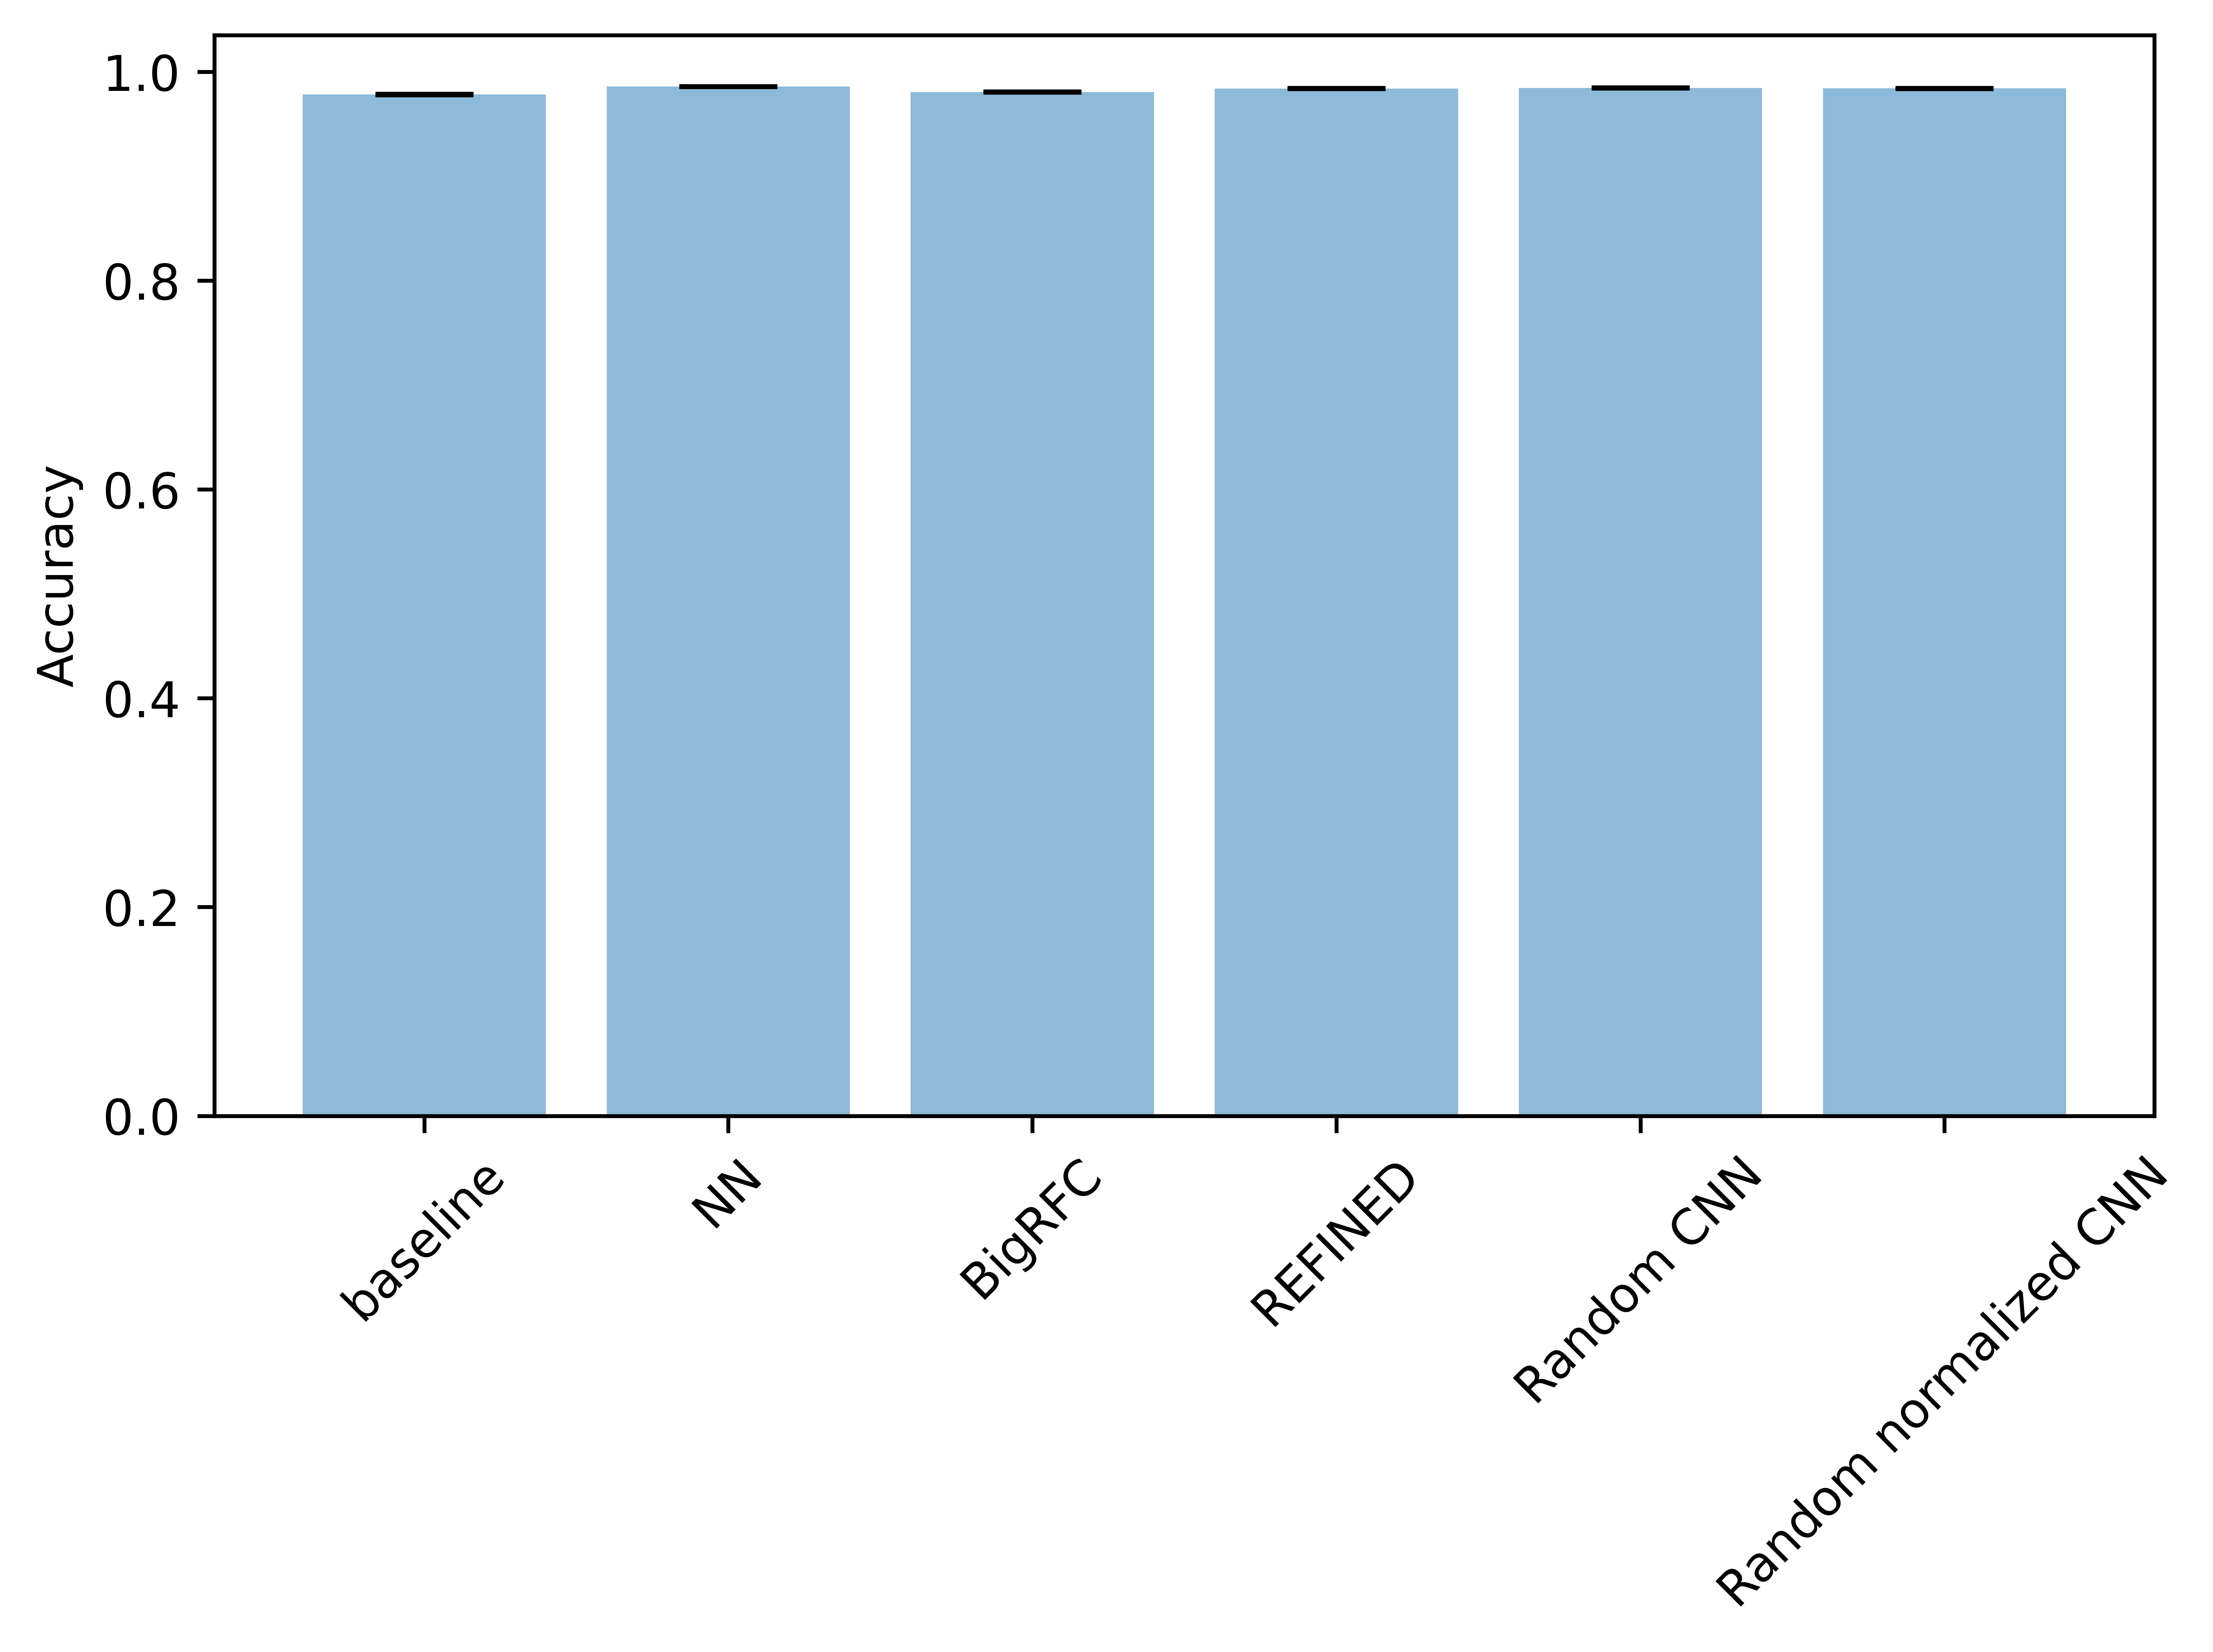
\includegraphics[width=0.5\linewidth]{img/Accuracy.png}
    \caption{Accuracy measurements for all models}
    \label{fig:accuracy}
\end{figure}
\begin{figure}
    \centering
    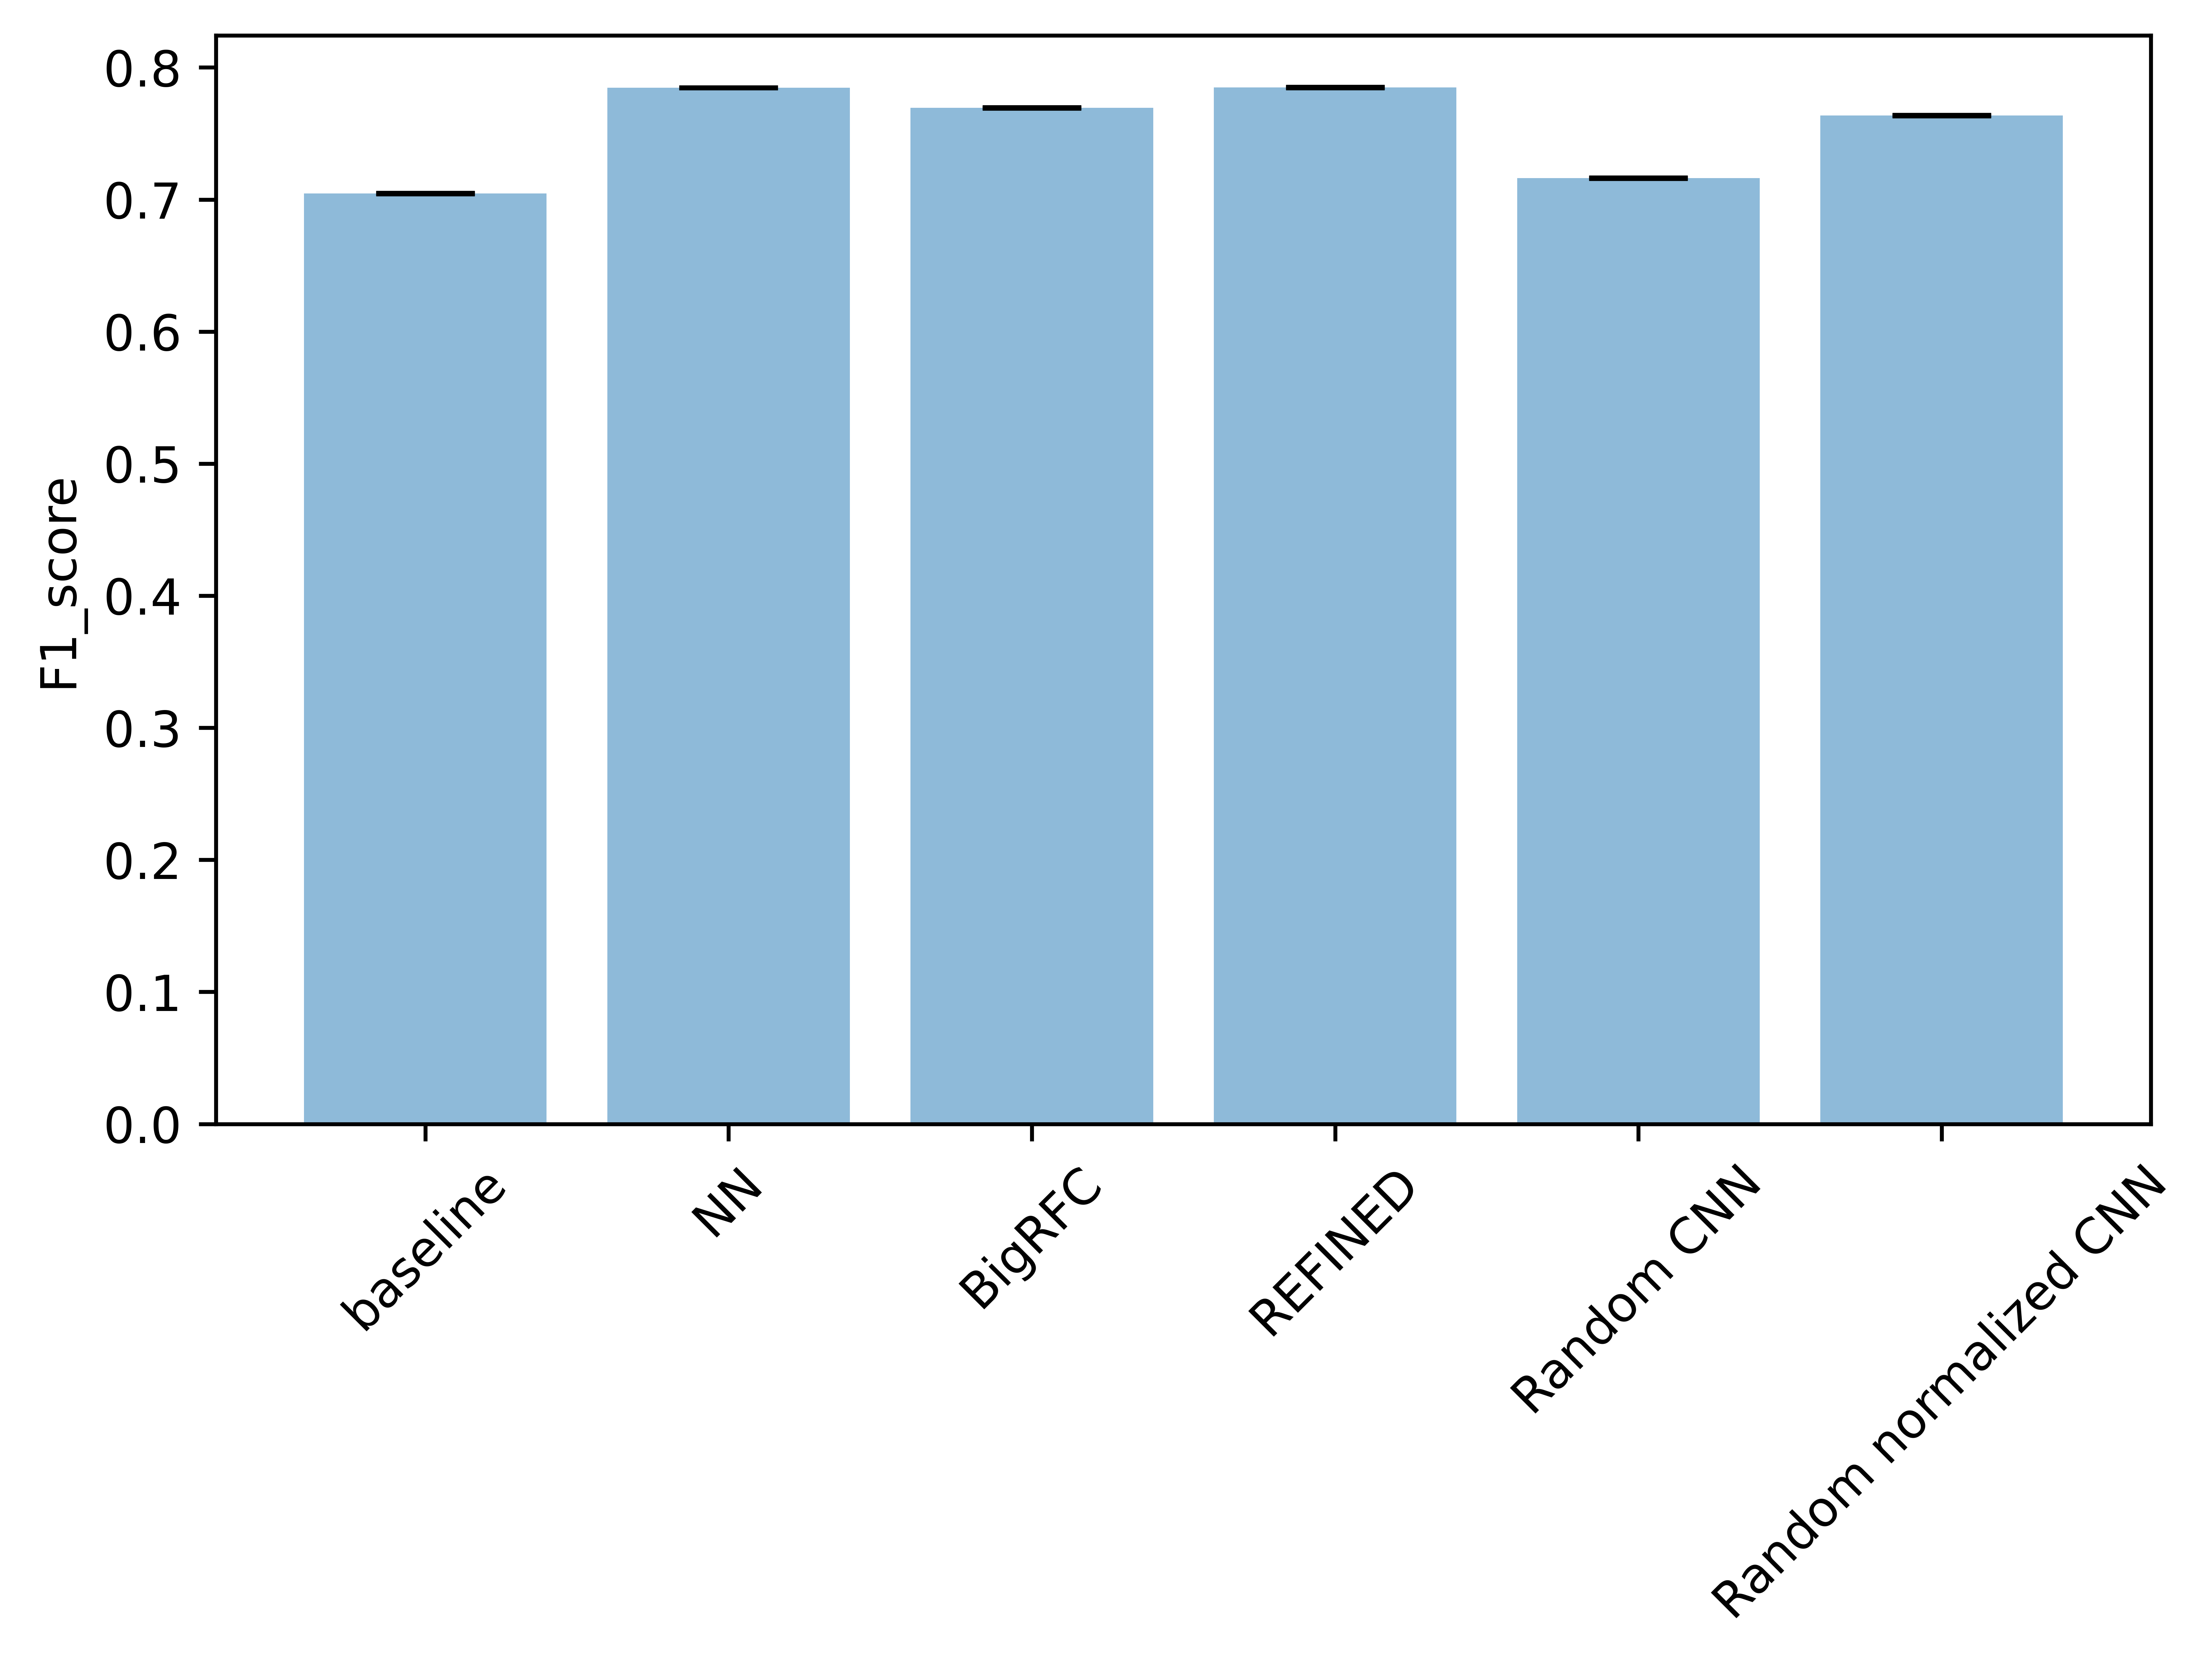
\includegraphics[width=0.5\linewidth]{F1_score.png}
    \caption{F1 scores for all models}
    \label{fig:f1}
\end{figure}

\begin{figure}
    \centering
    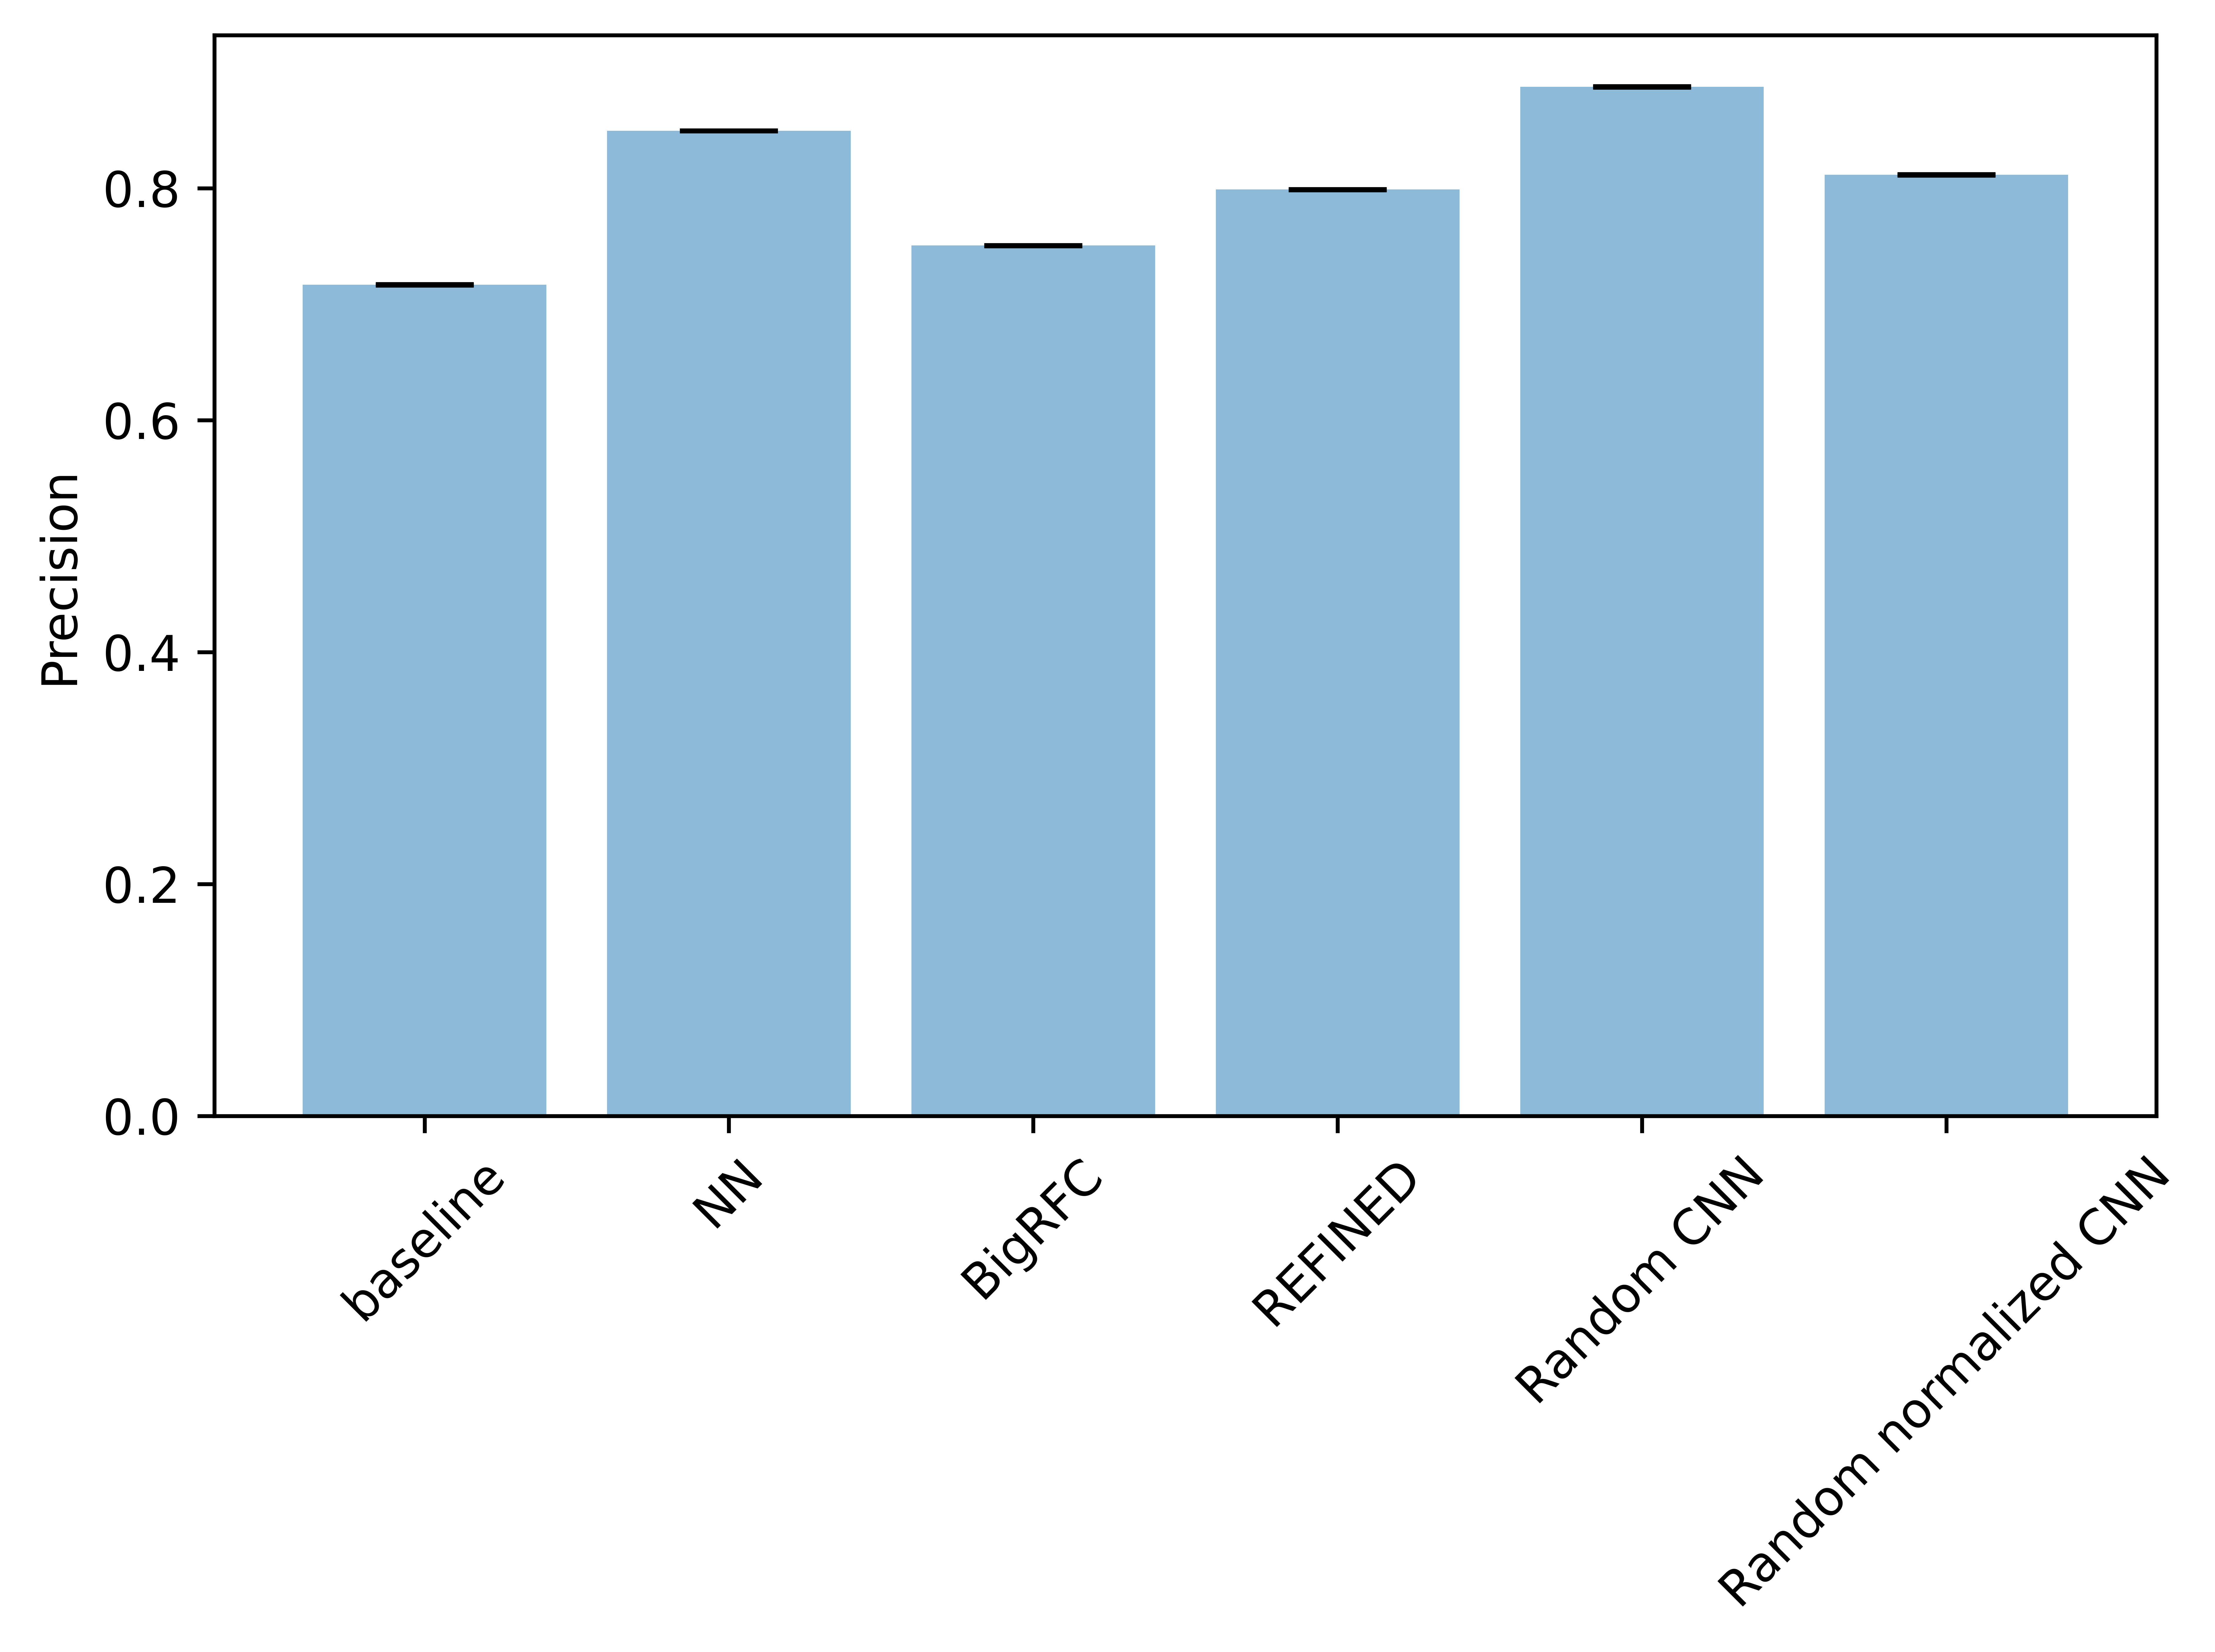
\includegraphics[width=0.5\linewidth]{Precision.png}
    \caption{Precision for all models}
    \label{fig:precision}
\end{figure}

\begin{figure}
    \centering
    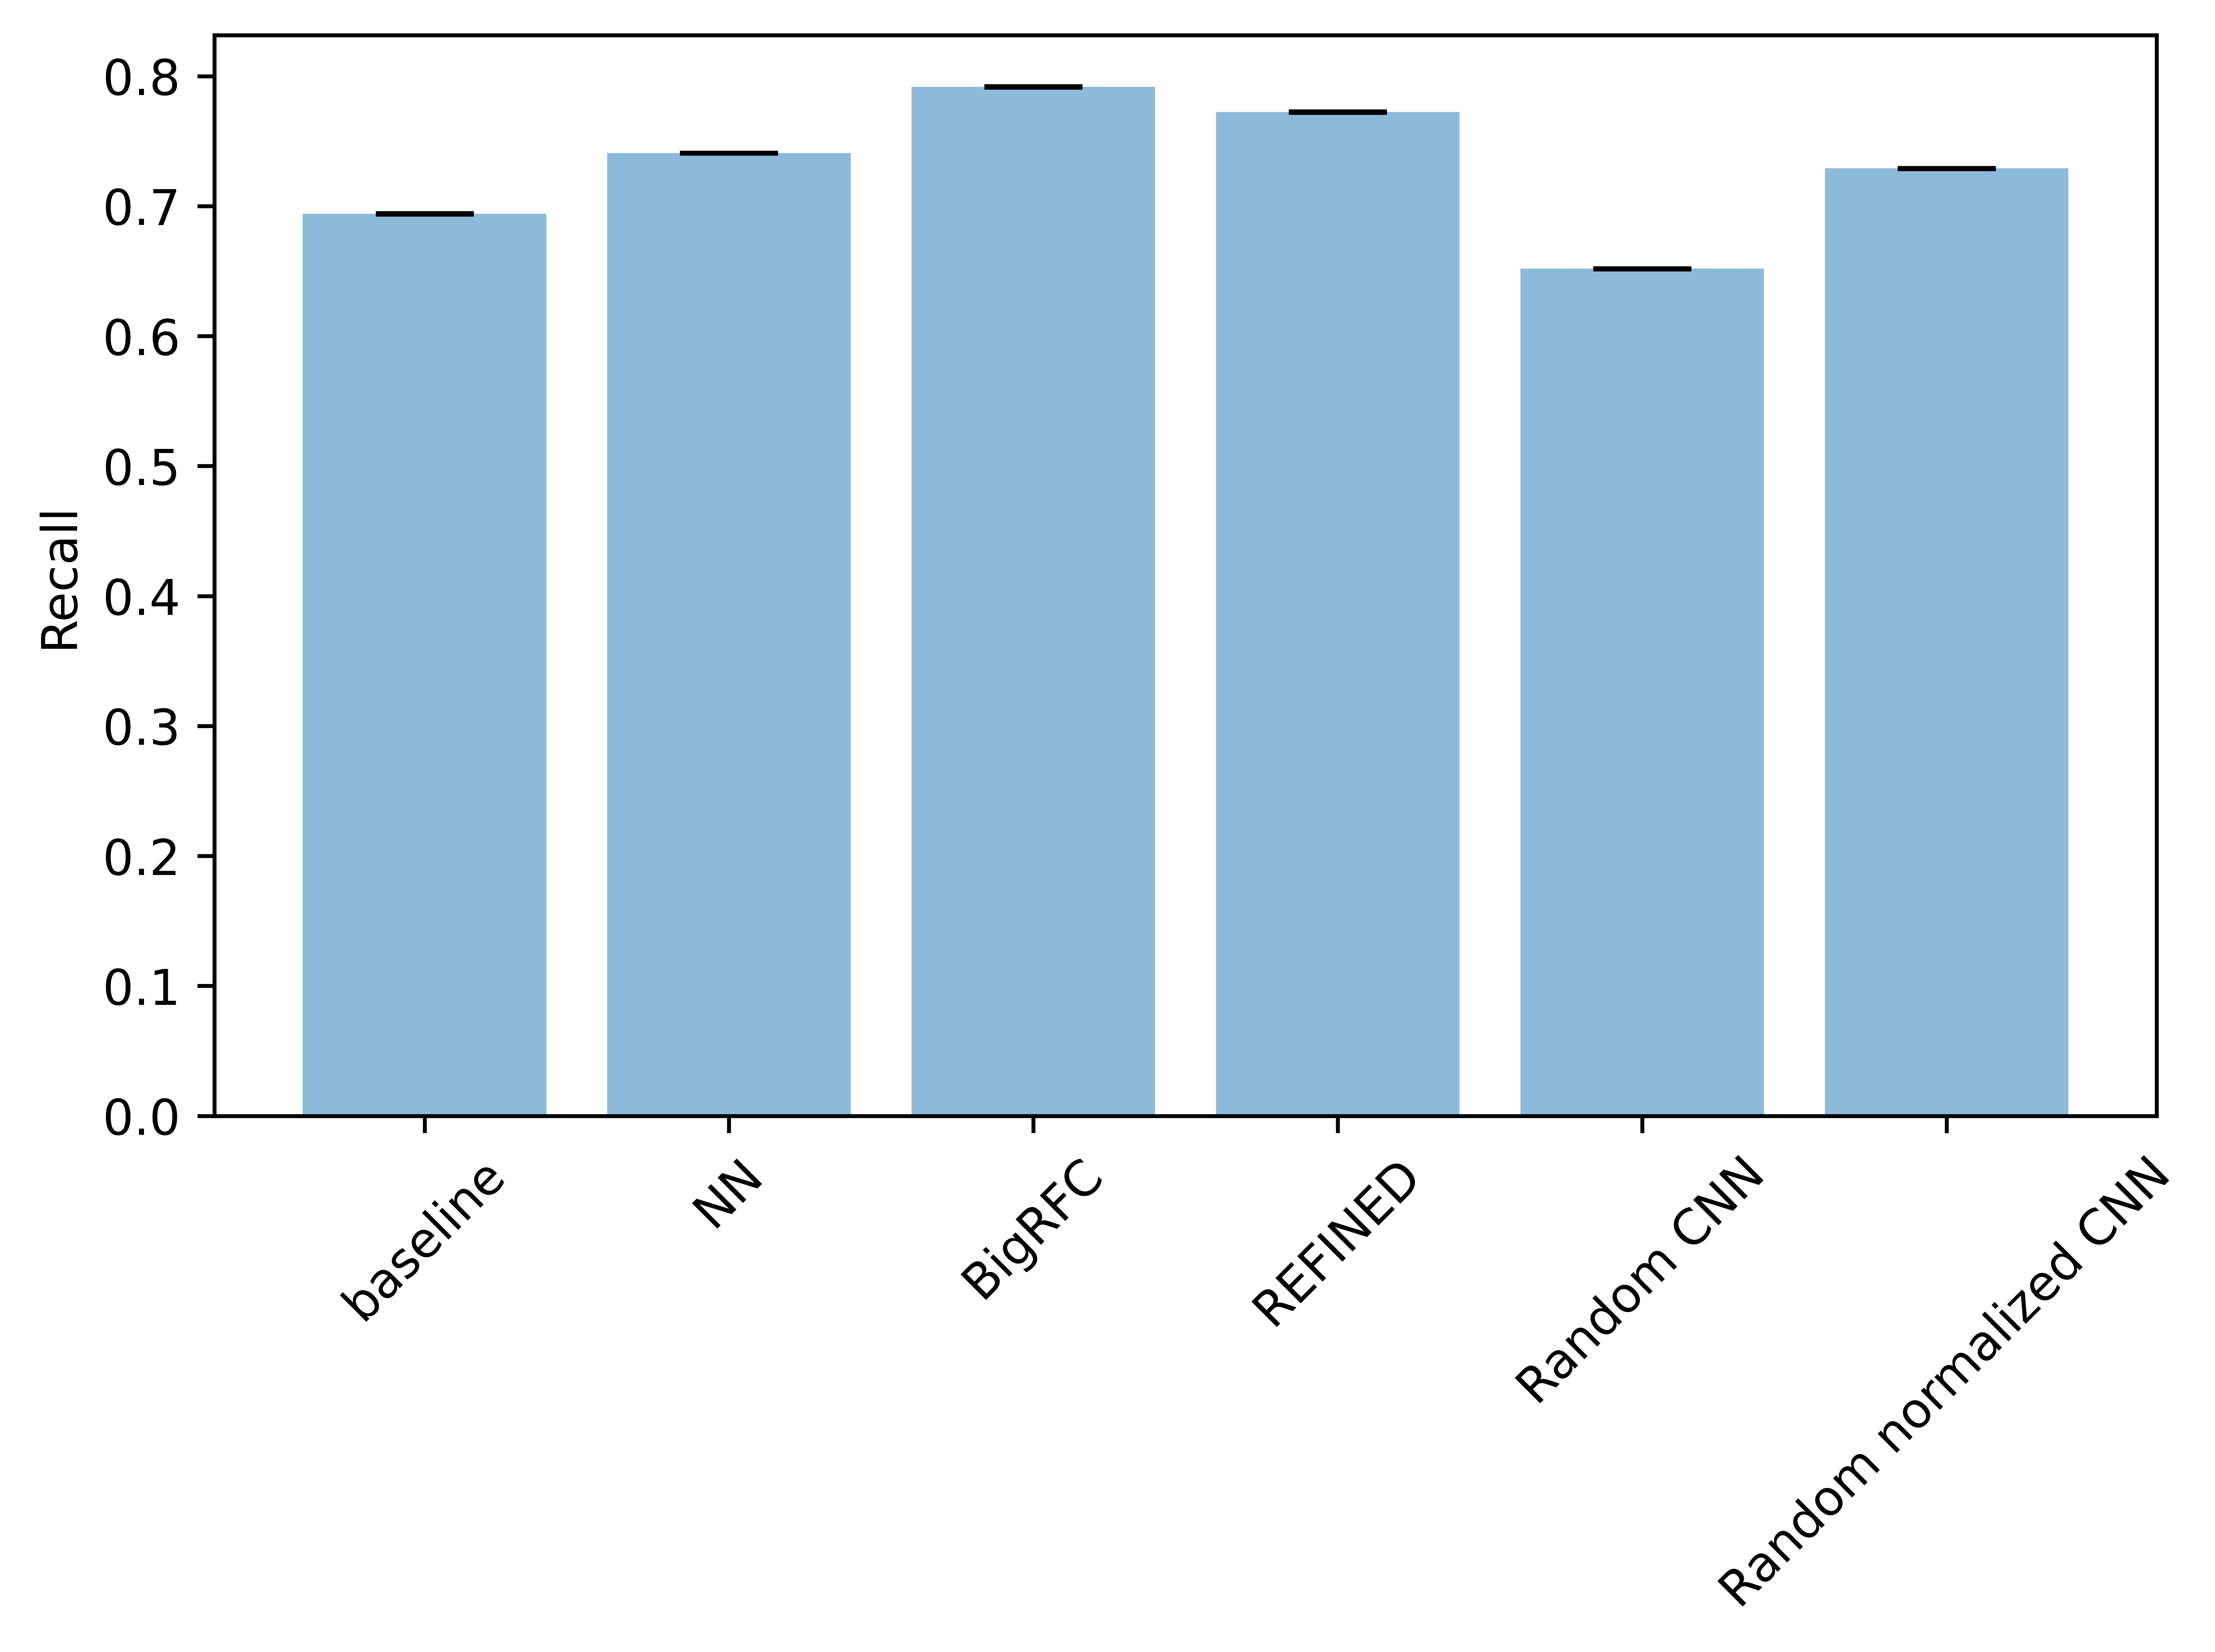
\includegraphics[width=0.5\linewidth]{Recall.png}
    \caption{Recall for all models}
    \label{fig:recall}
\end{figure}

As can be seen in the attached figures (~\ref{fig:accuracy}, ~\ref{fig:precision}, ~\ref{fig:f1}, ~\ref{fig:recall}) REFINED model is on par with state-of-the-art approaches, but does not bring higher performance as reported in \cite{REFINED}. However, it shows better results than Random CNN and even Random Normalized CNN.

\section{REFINED progression test}

With the negative results of the previous test, I wanted to test whether training a CNN on REFINED-transformed images produces better results than on images with randomly allocated positions. I have taken the individual epochs of REFINED and trained a CNN model on it to test this. The models are called \texttt{CNN-i}, where \texttt{i} is the number of epochs of REFINED used as input. So \texttt{CNN-0} will have features distributed very closely to randomly and \texttt{CNN-43} is a fully trained REFINED model. All of these models were trained using CNN hyperparameters found for the REFINED model in the first experiment.

Then, I tested whether there was any correlation between the REFINED score and CNN's performance. The obvious metric to compare is the validation loss, as it represents the training goals the best.

\begin{figure}
    \centering
    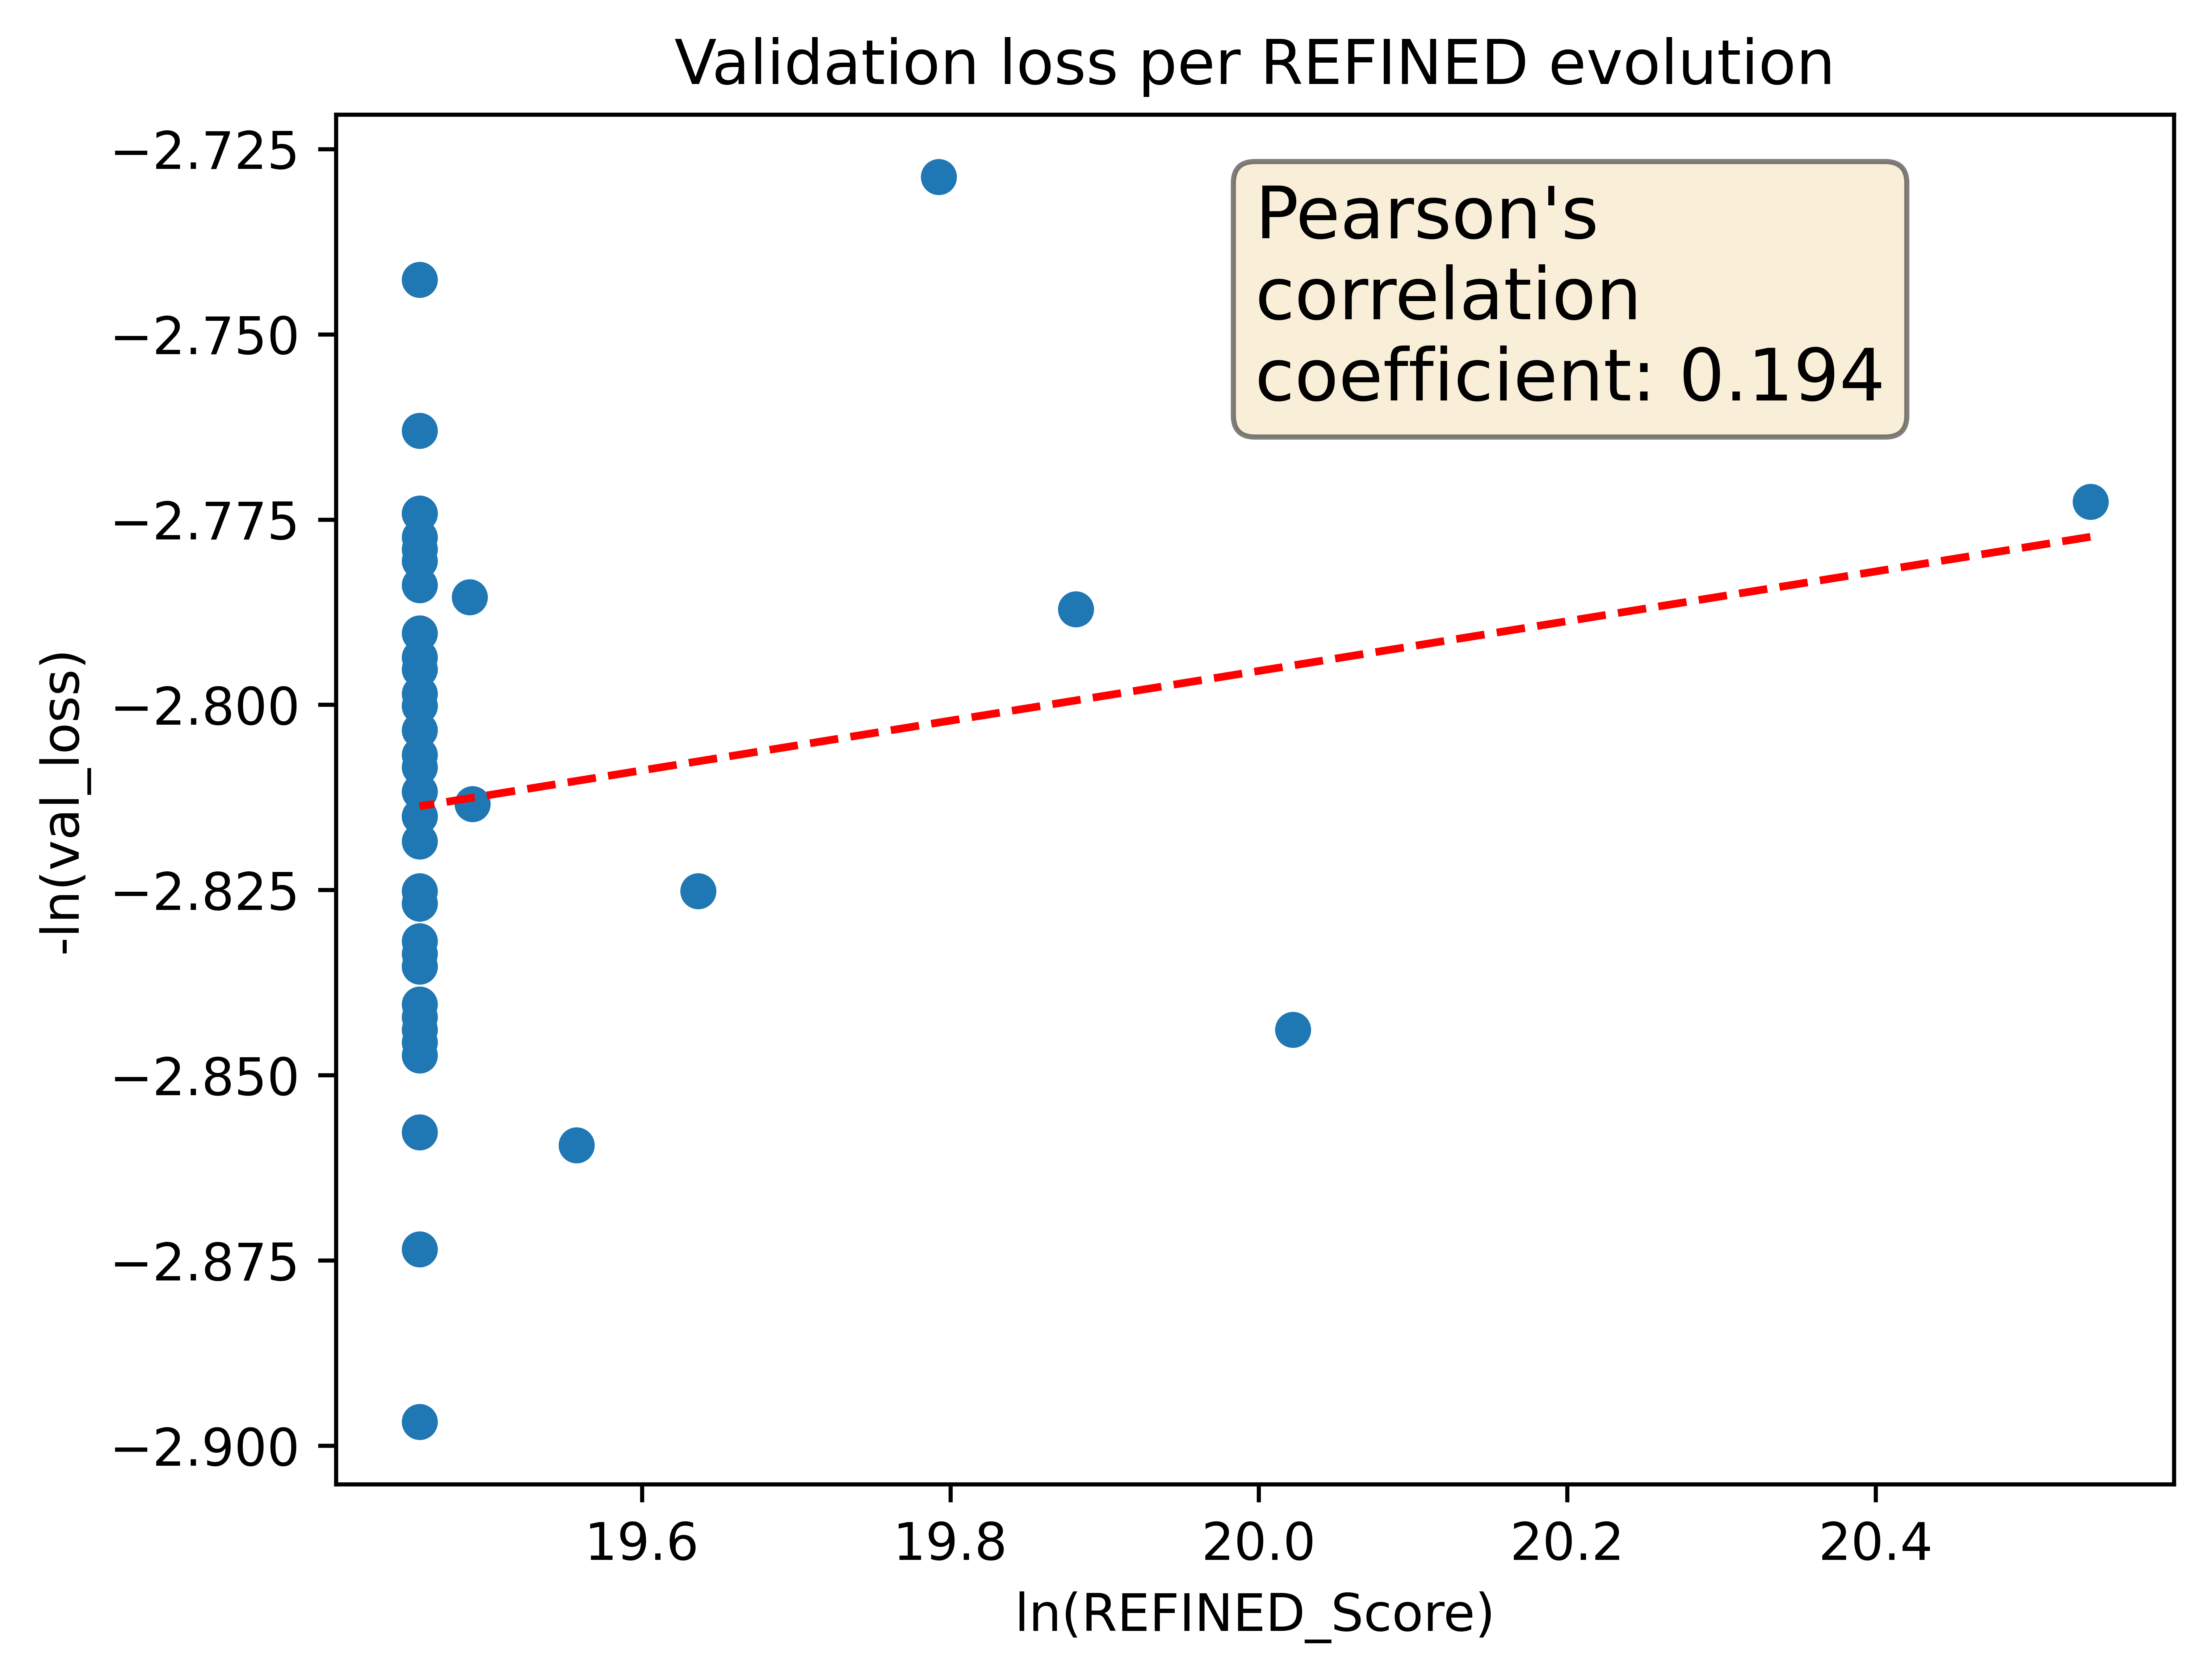
\includegraphics[width=0.5\linewidth]{progression.png}
    \caption{Best CNN validation loss plotted against }
    \label{fig:REFINED_progression}
\end{figure}

In ~\ref{fig:REFINED_progression} can be seen that there is little to no correlation between the REFINED score and the model's performance.

\section{REFINED transformation visualized}
At the beginning of this thesis, one of the motivations for this work was the interest in seeing high-dimensional data visualised in some manner. And REFINED does achieve that goal. 